\documentclass[9pt, xcolor=svgnames, dvipsnames]{beamer}
\usepackage[utf8]{inputenc}
\usetheme[progressbar=frametitle]{metropolis}
\usepackage{appendixnumberbeamer}
\usepackage{fancyvrb}
\usepackage{booktabs}
\usepackage[scale=2]{ccicons}
\usepackage{pgfplots}
\usepgfplotslibrary{dateplot}


\usepackage{xcolor}

\usepackage[export]{adjustbox}

%\usepackage{lmodern}
%\usepackage{tgbonum}
%\usepackage{tgcursor}
%\usepackage{courier}

\usepackage{type1cm}
\usepackage{yfonts, graphicx}
\usepackage{lettrine}
\usepackage[most]{tcolorbox}

%Python
\usepackage{minted}
\usemintedstyle{tango}





\usepackage{ragged2e}
\usepackage{xspace}
\usepackage{animate}
\newcommand{\themename}{\textbf{\textsc{metropolis}}\xspace}




\title[\mycode]{Programación en Python para Deep Learning\\ Introducción}
\subtitle{AI}

\usepackage{graphicx} % Allows including images
\usepackage{booktabs} % Allows the use of \toprule, \midrule and \bottomrule in tables

%\usepackage[utf8]{inputenc} %solucion del problema de los acentos.

\setbeamerfont{block title example}{size=\footnotesize}
%----------------------------------------------------------------------------------------
%TITLE PAGE
%----------------------------------------------------------------------------------------


\begin{document}
%\setminted[frame=lines, framesep=2mm, baselinestretch=1.2, bgcolor=LightGray, fontsize=\footnotesize]{python}
\newminted{python}{linenos=true, frame=lines, framesep=2mm, baselinestretch=1.2, bgcolor=LightGray, fontsize=\footnotesize}

\include{vars}

\author{J Peralta} % Your name
\institute[UNAB]{Universidad Andr\'es Bello}
% Date, can be changed to a custom date
\date{Viernes 10 de Junio 2022}

\begin{frame}
\titlepage % Print the title page as the first slide
\end{frame}

\begin{frame}
\frametitle{Resumen} % Table of contents slide, comment this block out to remove it
\tableofcontents % Throughout your presentation, if you choose to use \section{} and \subsection{} commands, these will automatically be printed on this slide as an overview of your presentation
\end{frame}


%----------------------------------------------------------------------------------------
%PRESENTATION SLIDES
%----------------------------------------------------------------------------------------
\metroset{block=fill}
%------------------------------------------------

%----------------------------------------------------------------------------------------
%PRESENTATION SLIDES
%----------------------------------------------------------------------------------------
%
%
%
\section{Una introducci\'on a Deep Learning \& Keras}

\begin{frame}[fragile]
\frametitle{?`Qu\'e es Deep Learning?}
\lettrine[lines=3]{\gothfamily\fontsize{50}{60}\scalebox{2}{U}}{na} definici\'on formal: \textit{Deep Learning (DL) es un subcampo de Machine-Learning (ML) en inteligencia artificial (AI) que trata con algoritmos inspirados desde la estructura biol\'ogica y funcionamienteo de un cerebro para ayudar a las m\'aquinas a tener inteligencia.}
\begin{itemize}
    \item Esto parece un nivel alto de dificultad para consumir en una sola frase.
    \item Lo primero es dividirlo en un set de distintos elementos.
    \item El orden espec\'ifico de subdivisi\'on es: DL, ML, e AI.
\end{itemize}
\end{frame}

\begin{frame}[fragile]
\frametitle{Desmitificar}
\textbf{AI} es una forma \textit{gen\'erica} que puede ser definida como la calidad de inteligencia introducida en maquinas. 

\begin{figure}
    \centering
    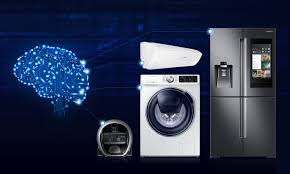
\includegraphics[width=0.6\textwidth]{Figuras/washing.jpeg}
\end{figure}


Las m\'aquinas usualmente son \textit{tontas}, entonces para hacerlas \textit{inteligentes} introducimos una \textit{especie} de inteligencia para que puedan tomar decisiones en forma independiente. Un ejemplo simple es una \textbf{lavadora autom\'atica}. La inteligencia de la m\'aquina \textbf{se introduce de forma artificial}, de ah\'i el nombre.
\end{frame}

\begin{frame}[fragile]
\frametitle{Desmitificar}
En este caso en particular de la lavadora, la \textit{inteligencia} es a\~nadida en la m\'aquina mediante un set de reglas \texttt{if-else}. Ac\'a el ingeniero pasa por todas las \textit{posibilidades}, y dise\~na el sistema en base a esas reglas.

\begin{figure}
    \centering
    
\includegraphics[width=0.6\textwidth]{Figuras/AI-ifelse.png}
\end{figure}
\end{frame}


\begin{frame}[fragile]
\frametitle{Desmitificar}

?`Qu\'e ocurre si necesitamos introducir inteligencia en una m\'aquina sin programar expl\'icitamente? ?`Algo que la m\'aquina pueda aprender por s\'i misma? \textit{Ac\'a es donde aparece el concepto de Machine Learning}

\begin{tcolorbox}
\textit{ML puede ser definido como el proceso de inducir inteligencia en un sistema o m\'aquina sin programaci\'on expl\'icita.}
\end{tcolorbox}

\begin{figure}
    \centering
    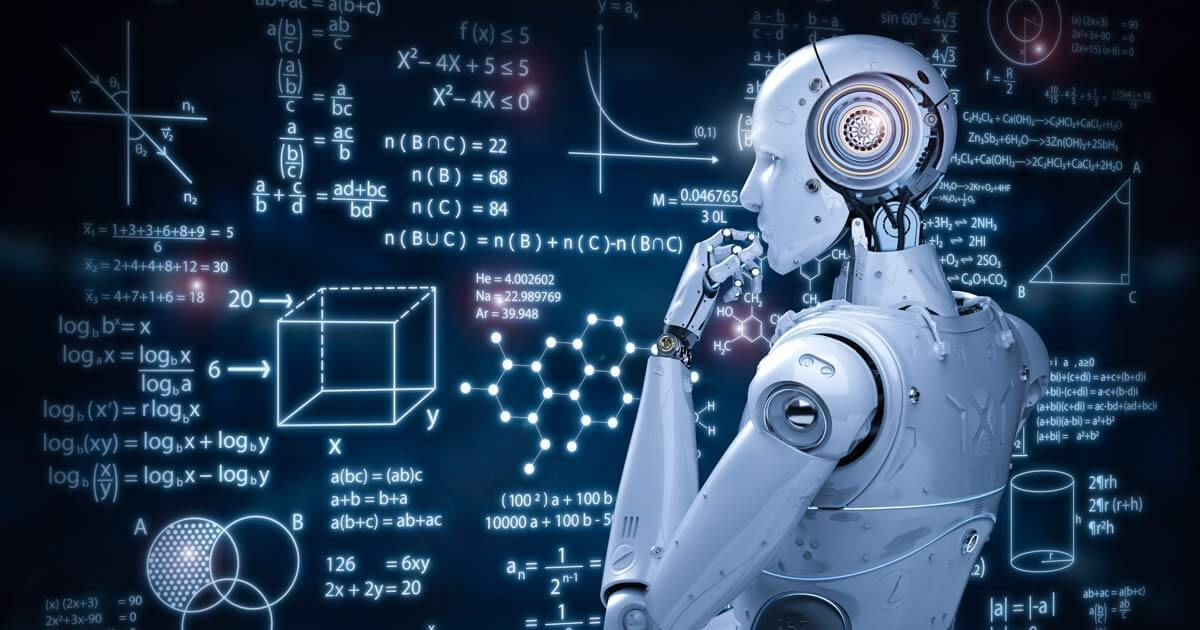
\includegraphics[width=0.6\textwidth]{Figuras/machine-learning-hearing-aid-article.jpg}
\end{figure}

\end{frame}

\begin{frame}[fragile]
\frametitle{Desmitificar}

Un ejemplo de ML, podr\'ia ser un sistema que puede predecir si un estudiante aprobar\'a o reprobar\'a en su siguiente examen en base a su \textit{comportamiento previo}.

?`Y DL donde aparece en este contexto? 

\begin{tcolorbox}
Ocurre que mientras ML trabaja muy bien para una gran variedad de problemas, este falla en casos espec\'ificos que son muy simples para los humanos, por ejemplo: clasificar una imagen como un gato o un perro; distinguir una voz femenina y una masculina; y muchas cosas m\'as.
\end{tcolorbox}

ML funciona mal para sistemas en que los tipos de datos \textbf{no} son estructurados.

\end{frame}


\begin{frame}[fragile]
\frametitle{Desmitificar}

Investigando las razones por las que ML no funcionaba bien en estos casos, apareci\'o una idea:

\begin{tcolorbox}
\textit{Imitar el proceso biol\'ogico del cerebro humano}. Es sabido que el cerebro es una orquesta de billones de neuronas conectadas que se adaptan para aprender nuevas cosas.
\end{tcolorbox}

\begin{figure}
    \centering
    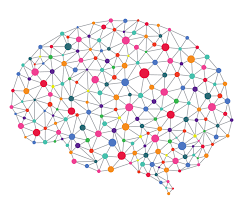
\includegraphics[width=0.4\textwidth]{Figuras/brain.png}
\end{figure}

\end{frame}

\begin{frame}[fragile]
\frametitle{Desmitificar}

Cuando la investigaci\'on uni\'o ML con estas redes neuronales, aparece el campo de Deep-Learning (DL), el que se enmarca en el desarrollo de Deep-Neural-Network (DNNs), que corresponde a redes neuronales de muchas capas. Ac\'a DL toma ventaja en donde ML no podr\'ia resolver el problema.

Todo esto ha ayudado a definir una nueva regla de oro: 
\begin{itemize}
    \item ML no mejorar\'a su performance cuando se incrementan datos de entrenamiento, luego de alcanzar cierto umbral.
    \item DL puede mejorar con m\'as datos, de manera m\'as eficiente para mejorar la performance.
\end{itemize}

\end{frame}




\section{Descomponiendo un modelo DL}

\begin{frame}[fragile]
\frametitle{Descomponiendo DL}
\begin{columns}
\begin{column}{0.4\textwidth}
\begin{itemize}\small
    \item En su forma b\'asica los modelos DL son dise\~nados usando redes neuronales.
    \item Una red es una organizaci\'on jer\'arquica de neuronas con conecci\'on a otras neuronas.
    \item Las neuronas pasan un mensaje o se\~nal a otras neuronas basadas en lo que reciben, y as\'i aprenden con alg\'un mecanismo de \textit{feedback}
    \item A la derecha hay una representaci\'on simplista de una red neuronal.
\end{itemize}
\end{column}
\begin{column}{0.6\textwidth}  %%<--- here
    \begin{center}
     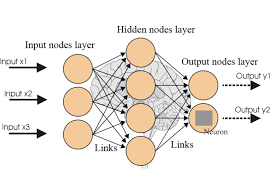
\includegraphics[width=1.0\textwidth]{Figuras/simplenn.png}
     \end{center}
\end{column}
\end{columns}
\end{frame}

\begin{frame}
\frametitle{Problemas cl\'asicos resueltos con DL}
\begin{columns}
\begin{column}{0.4\textwidth}
\begin{itemize}
    \item Sugerencias de etiquetado de rostros.
    \item Autom\'oviles independientes.
    \item Predicci\'on de la siguiente palabra al escribir.
    \item Alexa/Siri/Google Assistant.
    \item Reconocimiento de imagenes m\'edicas.
    \item Otros.
\end{itemize}
\end{column}
\begin{column}{0.6\textwidth}  %%<--- here
    \begin{center}
     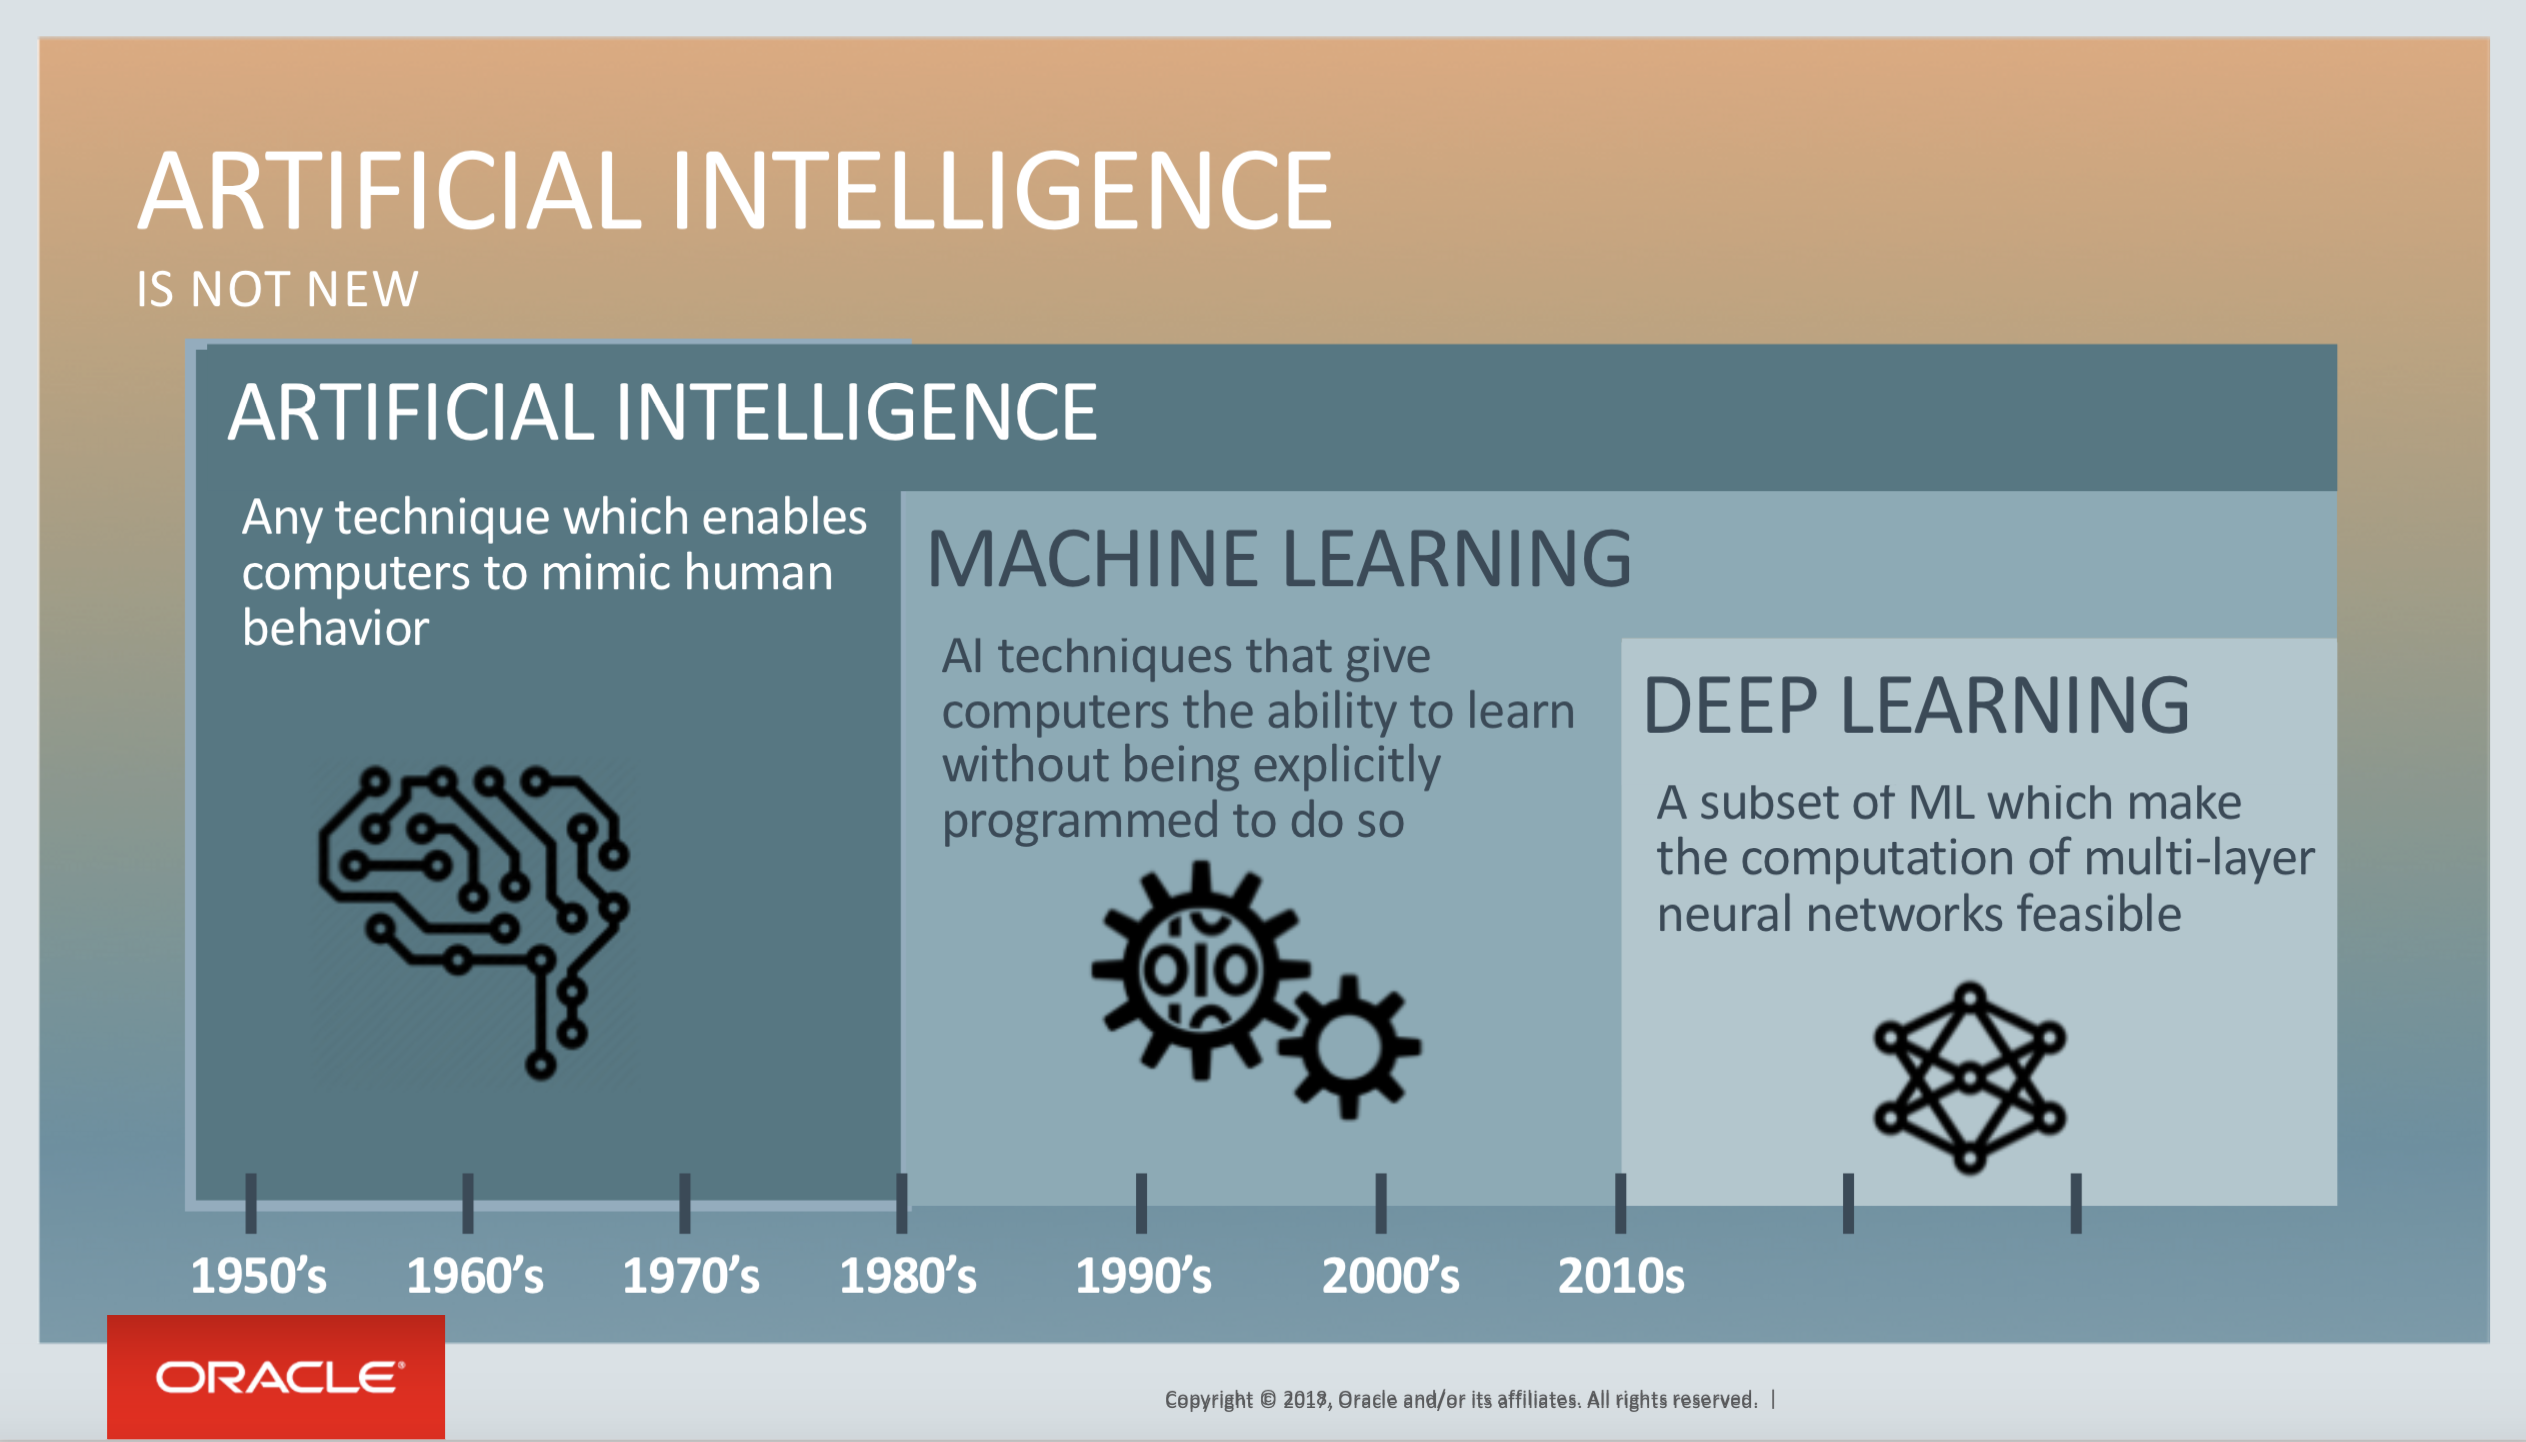
\includegraphics[width=1.0\textwidth]{Figuras/AIMLDL.png}
     \end{center}
\end{column}
\end{columns}
\end{frame}

\section{Marcos de Trabajo para DL}

\begin{frame}[fragile]
\frametitle{Marcos de Trabajo}
Existen dos marcos principales de trabajo para llevar a cabo estudios con DL (en Python3). Para ello tenemos disponible, programaci\'on de bajo y alto nivel.

\begin{tcolorbox}
Marcos de Bajo Nivel: Permiten programaci\'on m\'as espec\'ifica sobre elementos de las librer\'ias disponibles, funcionalidades propias de cada marco que permiten mayor flexibilidad, a un costo de incrementar la dificultad en la programaci\'on.
\end{tcolorbox}

\begin{tcolorbox}
Marcos de Alto Nivel: Permiten programaci\'on m\'as simple y general de DL, sin profundizar en los detalles de la programaci\'on que pueden o no ser accedidos, dependiendo el Marco en el que estemos trabajando.
\end{tcolorbox}
\end{frame}

\begin{frame}[fragile]
\frametitle{Marcos de Bajo Nivel}
\begin{itemize}
    \item Theano: Una de las primeras en ganar popularidad.
    \item Torch: Para ML y DL, Mejorada por Facebook.
    \item PyTorch: Desarrollado por Facebook AI Team para Python.
    \item MxNet: Desarrollado por distintas entidades, CMU, NYU, MIT, entre otros. Soporta multiples GPU, y provee a AWS, y Azure.
    \item TensorFlow: Una de las m\'as populares, desarrollada por Google para CPU, GPU y m\'obiles.
\end{itemize}    
\end{frame}

\begin{frame}[fragile]
\frametitle{Marcos de Alto Nivel}
\begin{itemize}
    \item Keras: Una de las m\'as Populares, escrita por y para Python. Funciona con Tensorflow, y otras.
    \item Gluon: Interface de alto nivel para mxnet.
    \item Lasagne: Interface de alto nivel para Theano.
\end{itemize}    
\end{frame}


\section{Una visita a Keras}

\begin{frame}[fragile]
\frametitle{Sneak Peek}
Observemos la siguiente DNN

\begin{center}
     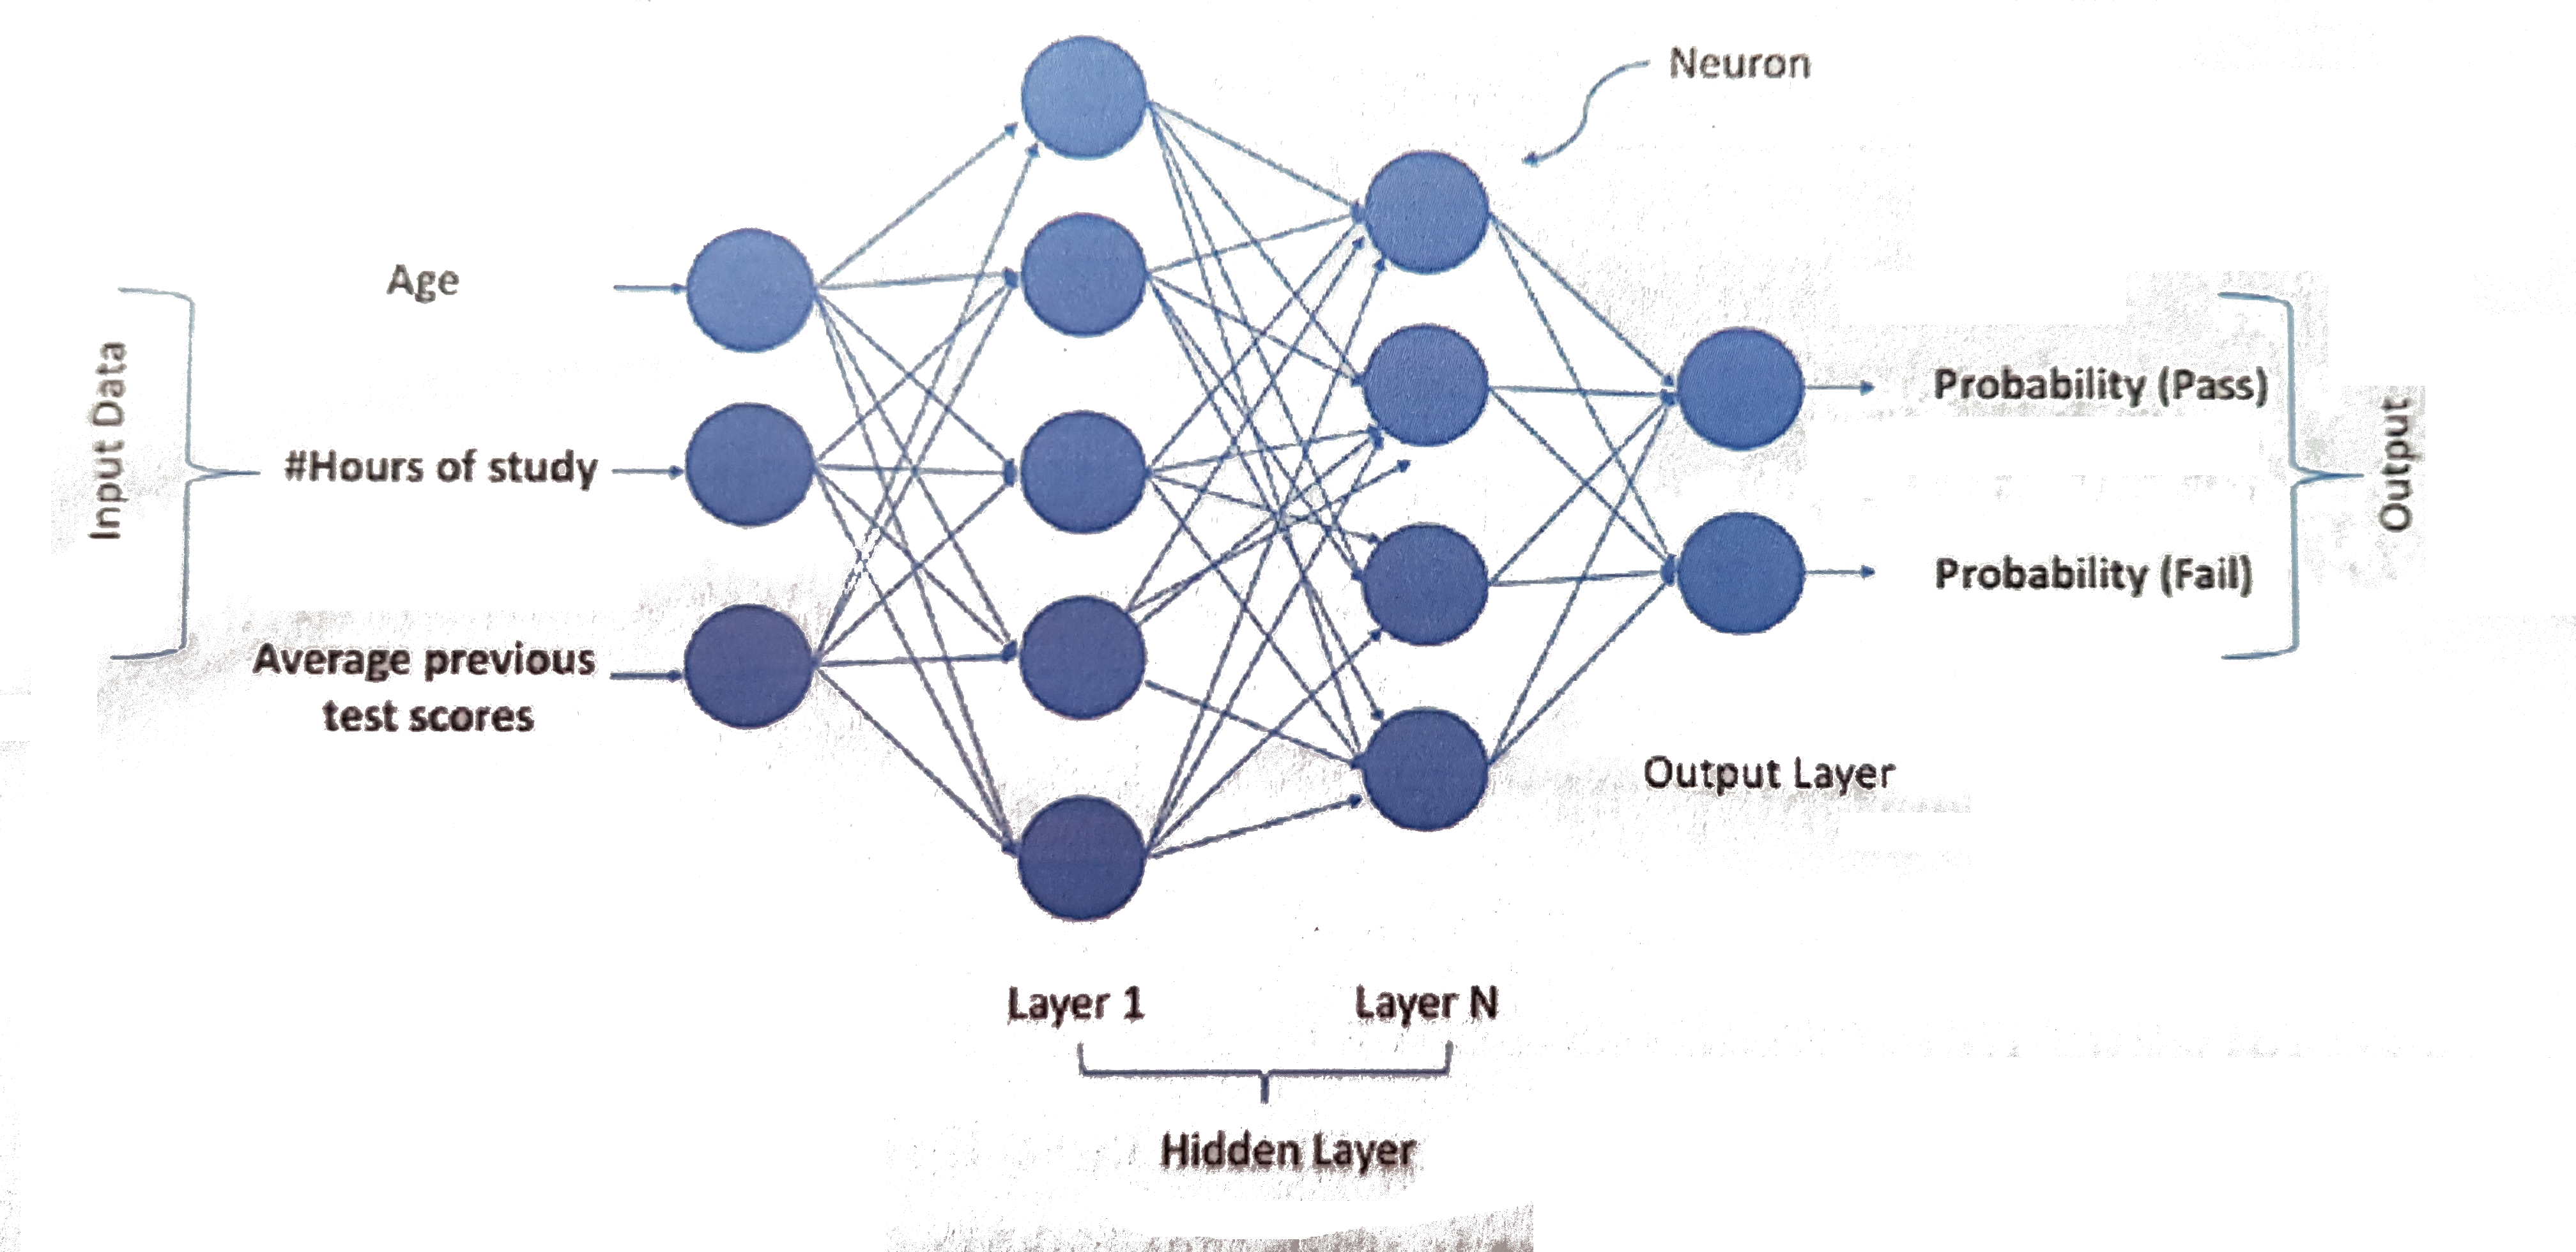
\includegraphics[width=1.0\textwidth]{Figuras/students.png}
\end{center}
\end{frame}

\begin{frame}[fragile]
\frametitle{El c\'odigo}
\begin{minted}[mathescape,fontsize=\scriptsize]{python}
from keras.models import Sequential
from keras.layers import Dense
import numpy as np

np.random.seed(2018)
#Edad/horas de esutdio/ promedio previo.
train_data, test_data = np.random.random((1000, 3)), np.random.random((500, 3)) 
labels = np.random.randint(2, size=(1000, 1)) #resultados de los examenes pass/fail

model = Sequential()
model.add(Dense(5, input_dim=3, activation='relu'))
model.add(Dense(4, activation='relu'))
model.add(Dense(1, activation='sigmoid'))
model.compile(loss='binary_crossentropy', optimizer='adam', metrics=['accuracy'])

model.fit(train_data, labels, epochs=10, batch_size=32)

predictions = model.predict(test_data)
\end{minted}
\end{frame}

\begin{frame}[fragile]
\frametitle{Data de Entrada}
Los datos de entrada pueden ser de distintos tipos, en general el modelo entiende los datos como \textit{tensores}. Lo que visto de forma simple, puede ser representado como una matriz $n-$dimensional.

\begin{table}[]
\begin{tabular}{
>|{\columncolor[HTML]{F8FF00}}|l|l|l} 
{\color[HTML]{32CB00} 1} & 5 & 3 & 1 & 1 \\
{\color[HTML]{32CB00} 2} & 4 & 5 & 1 & 2 \\
{\color[HTML]{32CB00} 3} & 4 & 6 & 8 & 9 \\
{\color[HTML]{32CB00} 4} & 5 & 5 & 6 & 7 \\
{\color[HTML]{32CB00} 5} & 9 & 1 & 6 & 9 \\
\end{tabular}
\end{table}
En esta tabla podemos representar los datos, por ejemplo tener $m$ columnas y $n$ filas. Ac\'a cada columna por defecto correspondera a una \textbf{muestra de entrenamiento}. Por ejemplo para el caso de los estudiantes, cada columna tendr\'ia 3 elementos, la edad, horas de estudio y promedio previo.
\end{frame}

\begin{frame}[fragile]
\frametitle{La Neurona}
La neurona es el core de DNN. Una neurona recibe uno o m\'as inputs desde capaz previas (o del dato crudo si corresponde a la primera capa).
\begin{center}
    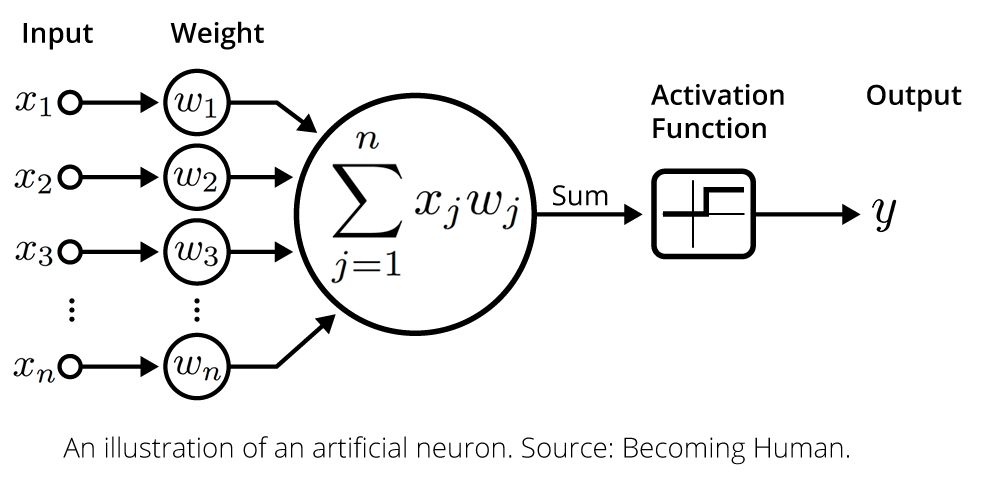
\includegraphics[width=0.7\textwidth, frame]{Figuras/neurona.png}
\end{center}

La \textit{funci\'on de activaci\'on} es vital en esta parte. Uno podr\'ia pensar ?`qu\'e ocurre si quitamos esta funci\'on? Lo primero es que el rango de salidas sería desde $-\infty$ hasta $\infty$ y no ser\'ia f\'acil definir un umbral. Además la red no aprendería, ya que en resumen la derivada de esta función sería 0 y esto impide el feedback en el aprendizaje.
\end{frame}

\begin{frame}[fragile]
\frametitle{Funciones de Activaci\'on}
\begin{center}
    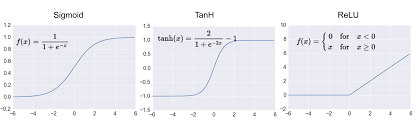
\includegraphics[width=0.7\textwidth, frame]{Figuras/activation.png}
\end{center}
Existen modificaciones en algunas de ellas, y se encuentran todas disponibles en Keras. Ahora que sabemos de modo general como funciona la neurona, entonces debemos proceder con construir un modelo adecuado para ellas.
\end{frame}

\begin{frame}[fragile]
\frametitle{El Modelo}
En Keras es posible crear apilamiento de capas mediante la a\~nadidura directa de ellas en un modelo general.

El modelo m\'as simple es el secuencial, que permite un apilamiento lineal de capas.

\begin{minted}[mathescape,fontsize=\normal]{python}
from keras.models import Sequential
from keras.layers import Dense, Activation

model = Sequential()
model.add(Dense(10, input_dim=15))
model.add(Activation('relu'))
\end{minted}
\end{frame}


\begin{frame}[fragile]
\frametitle{Capas}
Las capas est\'an definidas como grupos de neuronas, separadas de forma l\'ogica en una red jer\'arquica.Para simplificar el modelo Keras provee muchos tipos de capas y varias formas de conectarlas. Entr las principales se encuentran
\begin{itemize}
    \item Dense Layer: Una capa densa es una capa regular que conecta cada neurona definida en la capa, con cada neurona en la capa previa.
    \item Dropout Layer: Ayuda a reducir overfitting. Esta capa elimina unas pocas neuronas y reduce el calculo en el entrenamiento.
    \item Embedding layers / Convolutional layers / Pooling layers / etc.
    \item Uno puede incluso escribir su propia capa en Keras para un caso particular.
\end{itemize}
\end{frame}


\begin{frame}[fragile]
\frametitle{La funci\'on de p\'erdida}
Esta funci\'on es una m\'etrica que ayuda a la red a comprender si esta aprendiendo en la direcci\'on correcta.

Supongamos que tenemos las siguientes evaluaciones en cinco pruebas consecutivas: 3.8, 4.7, 5.5, 6.0, y 6.5. Uno podr\'ia pensar que esta mejorando el rendimiento ya que las notas suben. Si las notas bajan hubi\'esemos pensado lo contrario. De forma similar, la red utiliza una funci\'on para evaluar su desempe\~no.

\begin{tcolorbox}
En esencia la funci\'on de p\'erdida mide cuanto nos alejamos de un objetivo.
\end{tcolorbox}

Por ejemplo, para el caso de las notas y los estudiantes, nuestro modelo predice un puntaje de 0.87 para un alumno (1.0 aprueba / 0.0 reprueba). Si al modificar los pesos en nuestra red la predicci\'on baja a 0.4, entonces el cambio realizado no ayuda a aprender, y debemos deshacer este cambio. En cambio si sube a 0.9 entonces s\'i estar\'iamos aprendiendo en la direcci\'on correcta.

\end{frame}

\begin{frame}[fragile]
\frametitle{Algunas funciones de p\'erdida}
\begin{itemize}
    \item Mean Squared Error
    \item Mean Absolute Error
    \item Mean Absolute percentage error
    \item Mean Square logarithmic error
    \item Binary-cross entropy (por categor\'ia)
    \item Categorical cross-entropy (por categor\'ia)
\end{itemize}
\end{frame}

\begin{frame}[fragile]
\frametitle{Optimizadores}
Los optimizadores son la parte m\'as importante del modelo. Hasta ahora hemos hablado del feedback para el modelo, algoritmo llamado \textit{backpropagation}; este es en s\'i el optimizador.

Volvamos al modelo de estudiantes, e inicialicemos los pesos de los neuronas al azar en un principio. Al salir la señal luego de pasar por todas las capas, la función de pérdida nos dirá que tan bien esta el modelo (inicialmente al azar). Ahora el modelo, debe reducir esta función de perdida. ?`Pero cómo lo puede hacer el modelo? Acá es donde aparece el optimizador.

\begin{tcolorbox}
El optimizador es una funci\'on matem\'atica que usa derivadas, derivadas parciales, regla de la cadena y otros para comprender cuanto la red ver\'a en p\'erdida haciendo peque\~nos cambios al peso de las neuronas.
\end{tcolorbox}
\end{frame}

\begin{frame}
\frametitle{Optimizadores}
El c\'alculo de un entrenamiento de muestra desde el input al output es llamado un \textbf{pass}. Usualmente el entrenamiento se hace en \textbf{batches}, debido a los constrains de memoria de un computador.
\begin{tcolorbox}
Un batch es un subset de la muestra de entrenamiento completa.
\end{tcolorbox}

La red actualiza sus pesos luego de procesar un \textbf{batch} completo, esto es llamado una \textbf{iteration}.
\begin{tcolorbox}
Una vez que se han analizado todos los elementos de la muestra de entrenamiento, con su actualizaci\'on de pesos (batch by batch), tenemos lo que se conocer\'a como \textbf{epoch}.
\end{tcolorbox}

As\'i luego de muchos \textbf{epochs} la red aprendera a hacer predicciones cada vez m\'as correctas, en base a las muestras de entrenamiento dado.
\end{frame}

\begin{frame}
\frametitle{Optimizadores}
Entre los m\'as comunes se encuentran
\begin{itemize}
    \item Stochastic Gradient Descent (SGD)
    \item Adaptative Moment Estimation (Adam): Uno de los mejores actualmente.
    \item Adagrad
    \item Adadelta
    \item RMSPRop/ Adamax/ Nadam
\end{itemize}
\end{frame}

\begin{frame}
\frametitle{Metrica}
Similar a la funci\'on de p\'erdida, podemos definir la m\'etrica para el modelo. 

\begin{tcolorbox}
La metrica puede entenderse como la funci\'on usada para juzgar la performance del modelo sobre un set de datos no \textit{visto}, tambi\'en conocido como set de datos de validaci\'on.
\end{tcolorbox}

La diferencia principal de la m\'etrica con la fuci\'on de p\'erdida es que los resultados de la m\'etrica no son usados en el entrenamiento, s\'olo se usan para validar.
\end{frame}


\begin{frame}[fragile]
\frametitle{Configurando el modelo}
\begin{minted}[mathescape,fontsize=\scriptsize]{python}
from keras.models import Sequential
from keras.layers import Dense, Activation

model = Sequential()
model.add(Dense(32, input_dim=10, activation='relu'))
model.add(Dense(16, activation='relu'))
model.add(Dense(1, activation='sigmoid'))
model.compile(loss='binary_crossentropy', optimizer='adam', metrics=['accuracy'])

\end{minted}
\end{frame}

\begin{frame}[fragile]
\frametitle{Modelo completo}
\begin{minted}[mathescape,fontsize=\scriptsize]{python}
#Importa paquetes requeridos
from keras.models import Sequential
from keras.layers import Dense
import numpy as np

np.random.seed(2018)

x_train = np.random.random((6000, 10))
y_train = np.random.randint(2, size=(6000, 1))

x_val = np.random.random((2000, 10))
y_val = np.random.randint(2, size=(2000, 1))

x_test = np.random.random((2000, 10))
y_test = np.random.randint(2, size=(2000, 1))

model = Sequential()
model.add(Dense(64, input_dim=10, activation='relu'))
model.add(Dense(32, activation='relu'))
model.add(Dense(16, activation='relu'))
model.add(Dense(8, activation='relu'))
model.add(Dense(4, activation='relu'))
model.add(Dense(1, activation='sigmoid'))

model.compile(loss='binary_crossentropy', optimizer='adam', metrics=['accuracy'])

model.fit(x_train, y_train, epochs=10, batch_size=64, validation_data=(x_val, y_val))
\end{minted}
\end{frame}


\begin{frame}[fragile]
\frametitle{Evaluaci\'on del modelo}
?`Es un buen modelo? Hasta ahora no hemos distcutido si el modelo entregado es o no un buen modelo. 

Keras provee una funci\'on para evaluar el modelo, y testear.
\begin{minted}[mathescape,fontsize=\normal]{python}
print(model.evaluate(x_test, y_test))
\end{minted}
Eso mostrara algo como: \texttt{[0.6925000, 0.521]}. Lo que indica es el valor de la funci\'on de p\'erdida y la m\'etrica, si no recordamos qa que corresponden podemos usar: \texttt{print(model.metrics\_names)}. As\'i nuestro modelo da una presici\'on del 52\%, lo que es malo, pero es esperado ya que los n\'umeros fueron generados al azar.
\end{frame}

\begin{frame}[fragile]
\frametitle{Usando datos}
Vamos a un ejemplo m\'as completo, en base a un set de datos con informaci\'on sobre la diabetes en indio/americanos. Los datos se encuentran en este \href{https://raw.githubusercontent.com/jbrownlee/Datasets/master/pima-indians-diabetes.data.csv}{link}.

Las variables de estos datos son:

\begin{itemize}
    \item Input Variables (X):
    \begin{enumerate}
        \item Numero de ocaciones que se ha embarazado.
        \item Concentracion de glucosa a las dos hrs en test de tolerancia
        \item Presi\'on diast\'olica (mm Hg)
        \item Doblamiento (ancho) de piel de tr\'iceps (mm)
        \item Dos horas serum insulina (mu U/ml)
        \item \'Indice de masa corporal
        \item Diabetes pedigree function
        \item Edad
    \end{enumerate}
    \item Output Variables (y):
    \begin{enumerate}
        \item Clase (0 o 1)
    \end{enumerate}
\end{itemize}
Una vez que el archivo esta cargado, podemos dividir las columnas de datos en variables de entrada y salida.

\end{frame}


\begin{frame}[fragile]
\frametitle{El c\'odigo}
\begin{minted}[mathescape,fontsize=\scriptsize]{python}
# first neural network with keras make predictions
from numpy import loadtxt
from keras.models import Sequential
from keras.layers import Dense
# load the dataset
dataset = loadtxt('pima-indians-diabetes.data.txt', delimiter=',')
# split into input (X) and output (y) variables
X = dataset[:,0:8]
y = dataset[:,8]
# define the keras model
model = Sequential()
model.add(Dense(12, input_dim=8, activation='relu'))
model.add(Dense(8, activation='relu'))
model.add(Dense(1, activation='sigmoid'))
# compile the keras model
model.compile(loss='binary_crossentropy', optimizer='adam', metrics=['accuracy'])
# fit the keras model on the dataset
model.fit(X, y, epochs=150, batch_size=10)
print(model.evaluate(X, y))
\end{minted}
\end{frame}

\begin{frame}[fragile]
\frametitle{Predicci\'on con el modelo}
?`Y la predicci\'on?

Es f\'acil predecir con nuestro modelo, simplemente utilizando \texttt{predict} en nuestro c\'oidigo. 

En nuestro caso actual la salida es una funci\'on sigmoide entre 0 y 1, por lo que tenemos que normalizar para que nuestra predicci\'on sea el valor 0 o 1.

\begin{minted}[mathescape,fontsize=\scriptsize]{python}
# make probability predictions with the model
predictions = model.predict(X)
# round predictions 
rounded = [round(x[0]) for x in predictions]
\end{minted}

O bien, podemos hacerlo directament con:
\begin{minted}[mathescape,fontsize=\scriptsize]{python}
# make probability predictions with the model
predictions = model.predict_classes(X)
\end{minted}
\end{frame}

\begin{frame}[fragile]
\frametitle{La predicci\'on}
\footnotesize
\begin{verbatim}
...
Epoch 150/150
768/768 [==============================] - 0s 48us/step - loss: 0.4919 ...
[6.0, 148.0, 72.0, 35.0, 0.0, 33.6, 0.627, 50.0] => 1 (expected 1)
[1.0, 85.0, 66.0, 29.0, 0.0, 26.6, 0.351, 31.0] => 0 (expected 0)
[8.0, 183.0, 64.0, 0.0, 0.0, 23.3, 0.672, 32.0] => 1 (expected 1)
[1.0, 89.0, 66.0, 23.0, 94.0, 28.1, 0.167, 21.0] => 0 (expected 0)
[0.0, 137.0, 40.0, 35.0, 168.0, 43.1, 2.288, 33.0] => 1 (expected 1)
\end{verbatim}
    
\end{frame}


%------------------------------------------------
%------------------------------------------------
%------------------------------------------------
%------------------------------------------------
%------------------------------------------------
%------------------------------------------------
%------------------------------------------------
%------------------------------------------------
%------------------------------------------------
\begin{frame}
\begin{center}
\gothfamily\fontsize{50}{60}\scalebox{2}{Fin}
\end{center}
\end{frame}

%----------------------------------------------------------------------------------------


\end{document} 
